\documentclass[12pt,a4paper]{article}
\usepackage[utf8]{inputenc}
\usepackage[english]{babel}
\usepackage[T1]{fontenc}
\usepackage{amsmath}
\usepackage{amsfonts}
\usepackage{amssymb}
\usepackage{graphicx}
\usepackage{siunitx}
\usepackage{float}
\usepackage[left=2cm,right=2cm,top=2cm,bottom=2cm]{geometry}
\author{Gerald}

\begin{document}
\sisetup{separate-uncertainty = true}
	\setlength{\parindent}{0pt} 
	\begin{center}
		{\LARGE Experiment protocol}\\
		\begin{large}
			for the solid state lab course\\[0.4cm]
			at RWTH Aachen\\
			II. Physikalisches Institut A\\[5.5cm]
			\Large\textbf{\textsl{Superconductivity and SQUID}}\\[5.5cm]
			\normalsize\textit{authored\\by}\\[0.4cm]
			\large{Moritz Berger (355244)\\Gerald Kolter (355005)}\\[2cm]
			\large \textbf{Summer term 2019}
		\end{large}
	\end{center}
	\newpage
	
	\tableofcontents
	\newpage

\section{Introduction}
Superconducting Quantum Information Devices ("SQUIDS") are very sensitive sensors for measuring changes in the magnetic field. A SQUID consists of a ring shaped superconductor with two contacts and one Josephson junction on each path between the contacts. A Josephson junction is a small insulator disrupting the  superconductor. Electrons can tunnel through the insulator as Cooper pairs. \\
The resolution of the measured magnetic flux is in the order of the so called fluxonium or flux quantum:
\begin{equation*}
\Phi _0 = \dfrac{h}{2e} = \SI{2.07e-15}{Wb}
\end{equation*}
Only a complete flux quantum can penetrate the ring. If the surrounding field is not exactly a multiple of the flux quantum a current gets induced into the superconductor, that increases/decreases the field strength to a full quantum. This current can be measured.


\section{Goal of the Experiment}

The goal of the experiment is to determine the value of the flux quantum.
To achieve this the critical temperature of the superconducting material $T_C$ is determined in a first step.. \\
With the SQUID cooled down to the superconducting regime one measures the voltage-current characteristic. From this one can determine the critical current $I_C$, the resistance in the normal conducting state $R_N$ and the characteristic voltage $V_C$. \\
Next one measures the voltage-magnetic flux characteristic. From this one determines the SQUID parameter $b_L$ given by:
\begin{equation}
b_L = 2 \cdot I_C \cdot \dfrac{L}{\Phi _0}
\end{equation}
And with that the magnetic flux quantum $\Phi _0$. \\
With bringing different metallic objects in the vicinity of the SQUID one can demonstrate the sensitivity of the SQUID to external magnetic fields. This is done with and without the metallic shielding of the SQUID.


\section{Setup}
The setup consits of a SQUID in a metallic tube, which shields external magnetic fields. The setup is called "Mr. SQUID" and selled by the company "Conductus". The SQUID is sinked in a dewar filled with liquid nitrogen to cool it down to the necessary temperatures. \\
The SQUID itself is build out of Yba$_2$Cu$_3$O$_{7-x}$ with $x \approx 0-0.2$. The temperature is measured with a Pt-100 resistor.


\section{Temperature Calibration}
\subsection{Measurement}
The temperature is measured with a Pt-100 resistor, which measures a resistance. For the calibration the resistance at room temperature, measured with a thermometer, and at the temperature of the liquid nitrogen. For this the SQUID including the resistor is sinked into the liquid nitrogen and the resistance is measured after it stabalized. In this area a linear dependence between the resistance and the temperature is assumed.

\subsection{Data}

\begin{figure} [H]
\centering
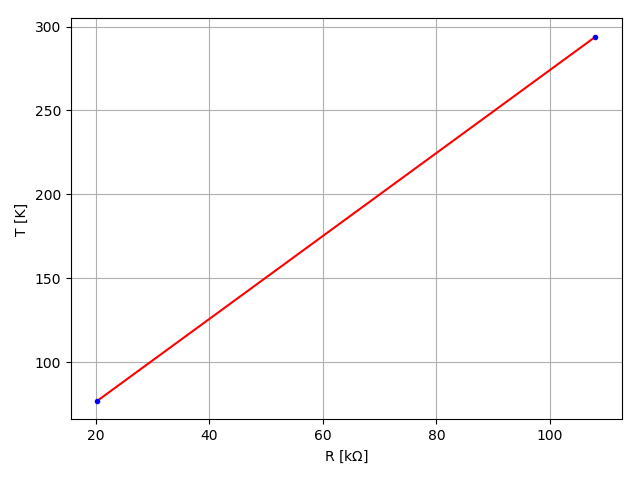
\includegraphics[scale=0.8]{Bilder/Temp_kalibration.PNG}
\caption{Temperature calibration for the Pt-100 resistor.}
\label{fig:Temp_kalibration}
\end{figure}

Fig. \ref{fig:Temp_kalibration} shows the calibration. The two points are the two measurements and the orange line is the linear calibration. 

\subsection{Results}

\begin{table} [H]
\centering
\begin{tabular}{|c|c|c|c|}
\hline 
$T_{room}$ [K] & $T_{LN_2}$ [K] & $R_{RT}$ [k$\Omega$] & $R_{LN_2}$ [k$\Omega$] \\ 
\hline 
294.65 $\pm$ $\frac{1}{\sqrt{12}}$ & 77 $\pm$ $\frac{1}{\sqrt{12}}$ & 107.9 $\pm$ $\frac{1}{\sqrt{12}}$ & 20.3 $\pm$ $\frac{1}{\sqrt{12}}$ \\ 
\hline 
\end{tabular} 
\caption{Measured values for the resistance at room temperature and the temperature of liquid nitrogen.}
\label{tab:Temp_Calib_data}
\end{table}

For a measured resistance from the Pt-100 resistor $R_{measured}$ one can calculate the temperature with:
\begin{equation*}
T = \dfrac{T_{room} - T_{LN_2}}{R_{RT} - R_{LN_2}} \cdot R_{measured} + T_{room} - \dfrac{T_{room} - T_{LN_2}}{R_{RT} - R_{LN_2}} \cdot R_{RT}
\end{equation*}
With $R_{RT}$ being the resistance measured at room temperature, $R_{LN_2}$ the resistance at the temperature of liquid nitrogen, $T_{room}$ the room temperature and $T_{LN_2}$ the temperature of liquid nitrogen. We assume the same error on all resistance measurements $\sigma _R = \frac{\SI{1}{k \Omega}}{\sqrt{12}}$ and the same error on all temperature measurements $\sigma _T = \frac{\SI{1}{K}}{\sqrt{12}}$.


\section{Temperature Dependence of the Resistance}
\subsection{Measurement}
The voltage in dependence of the current is measured while the sample is slowly cooled down. For that purpose the sample is moved down slowly in the dewar while not being in contact with with the liquid nitrogen.

\subsection{Data}

\begin{figure} [H]
\centering
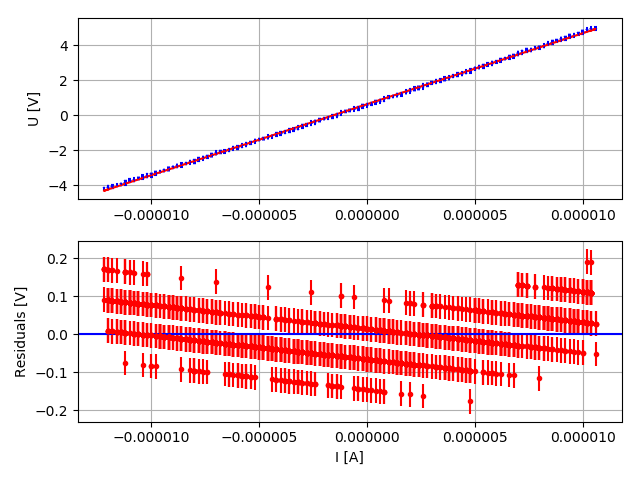
\includegraphics[scale=0.8]{Bilder/Critical_Temperature/Resistance_fit_13.PNG}
\caption{SQUID voltage in dependence of the current at \SI{237 \pm 2}{K}.}
\label{fig:Temp_Resistance_example}
\end{figure}

Fig. \ref{fig:Temp_Resistance_example} shows exemplary one of the measured curves for the SQUID voltage in dependence of the current at \SI{237 \pm 2}{K}. The slope yields the resistance of the SQUID at that point so its extracted with a linear fit, which is already done in the shown plot.

\subsection{Results}

\begin{figure} [H]
\centering
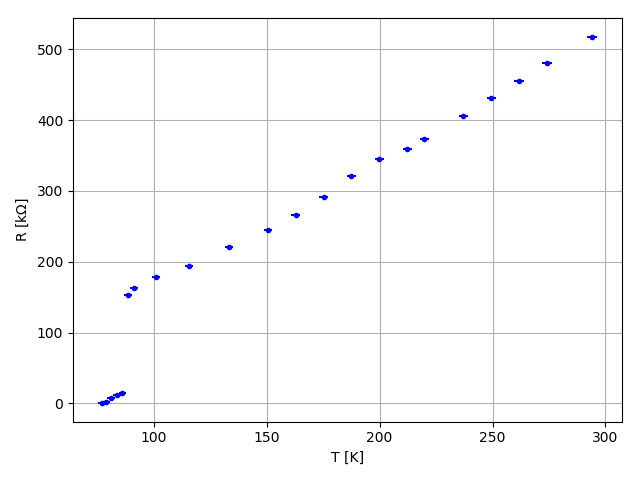
\includegraphics[scale=0.8]{Bilder/Critical_Temperature/Temp_Resistance.PNG}
\caption{SQUID resistance in dependence of the temperature.}
\label{fig:Temp_Resistance}
\end{figure}

Fig. \ref{fig:Temp_Resistance} shows the completed plot of the resistance vs. the temperature. As expected there is a big drop in the resistance at a certain temperature. \\
The critical temperature at which the resistance drops can be read off by taking the two points limiting the drop, i.e. the lowest point above and the highest below the drop. The critical temperature is estimated by the mean value of these two and the error by the difference devided by $\sqrt{12}$. This leads to the value:
\begin{equation*}
T_C = \SI{87.39 \pm 0.71}{K}
\end{equation*}


\section{U-I-Characteristic}
\subsection{Measurement}
With the sample submerged in liquid nitrogen and after temperature stabilization the U-I-Characteristic characteristic is measured. This is done by recording the applied current and the resulting voltage with an oscilloscope.

\subsection{Data}

\begin{figure} [H]
\centering
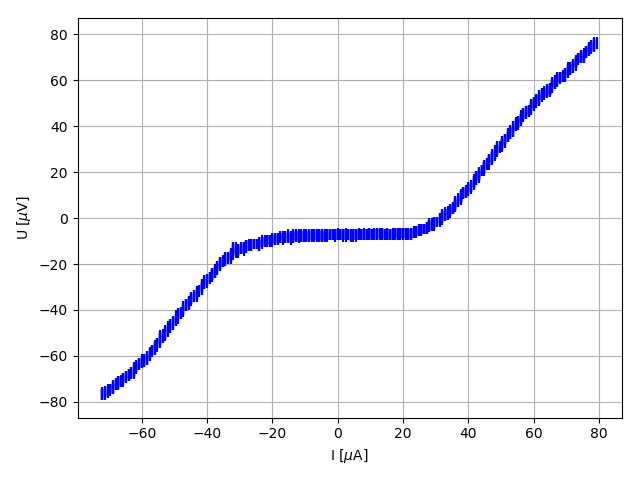
\includegraphics[scale=0.8]{Bilder/U_I_characteristic/characteristic.PNG}
\caption{U-I characteristic of the SQUID in the superconducting state.}
\label{fig:U-I-characteristic}
\end{figure}

Fig. \ref{fig:U-I-characteristic} shows the U-I characteristic of the SQUID in the superconducting state. As expected one can see a plateau around zero current. Outside from that one sees a linear dependence.

\subsection{Results}

\begin{figure} [H]
\centering
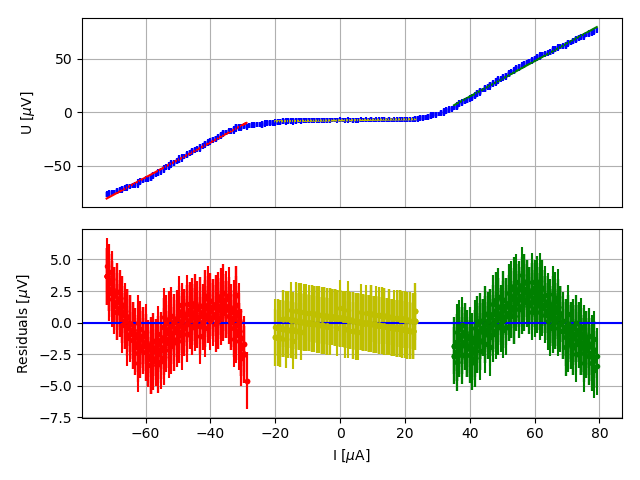
\includegraphics[scale=0.8]{Bilder/U_I_characteristic/fit_43.PNG}
\caption{U-I characteristic of the SQUID in the superconducting state.}
\label{fig:U-I-characteristic_fit}
\end{figure}

The critical current of the SQUID is equal to half of the width of the plateau. To determine this width one fits three linear regimes: One on the plateau and one each before and after it. Fig. \ref{fig:U-I-characteristic_fit} shows the U-I characteristic and the three fits. \\
The width of the plateau is the distance in x direction between the two cross sections between the fit at the plateau and each of the other one. This yields the result:
\begin{equation*}
I_C^{SQUID} = \SI{27.79 \pm 0.21}{\mu A}
\end{equation*}
The error is determined by propagating the errors coming from the fits. \\
\\
From the two linear fits in before and after the plateau one get the SQUID resistance in the normal conductive regime $R_N$ which is equal to the slope. The result is the averaged mean between these two:
\begin{equation*}
R_N^{SQUID} = \SI{16458 \pm 54}{\Omega}
\end{equation*}\\
\\
With the critical current and the resistance in the normal conductive regime one can calculate the characteristic voltage:
\begin{equation*}
V_C^{SQUID} = \SI{0.4574 \pm 0.0037}{V}
\end{equation*}\\
\\
As the SQUID consists of two identical Josephson junctions one can easily calculate the corresponding values for one Josephson junction:
\begin{equation*}
I_C^{JJ} = \SI{13.89 \pm 0.10}{\mu A} \qquad R_N^{JJ} = \SI{32916 \pm 108}{\Omega}
\end{equation*}


\section{U-$\si{\phi}$-characteristic}

\subsection{Measurement}
The U-$\si{\phi}$-characteristic is measured by changing the applied flux instead of the current and again measuring the voltage similar to the U-I-characteristic.


\subsection{Data}
The oscilloscope picture and the resulting U-$\si{\phi}$-characteristic can be seen in figure \ref{fig:U-phi_data}. The flux is not actually calibrated and instead the voltage change is displayed on the x-axis. One can see the periodic dependence of the voltage on the applied flux. However the periodicity is not constant in the U-$\si{\phi}$-plot and instead changes to shorter periods at higher applied flux. This is a result of the measured flux not being increased linearly. The oscillations depended on time, which are measured by the oscilloscope, do not reflect this non-linearity, because they already have a constant period (which would mean a linear increase). For this reason the U-$\phi$-plot is not used for the analysis and instead everything is analyzed with the U-t-plot of the oscilloscope.

\begin{figure}
\centering
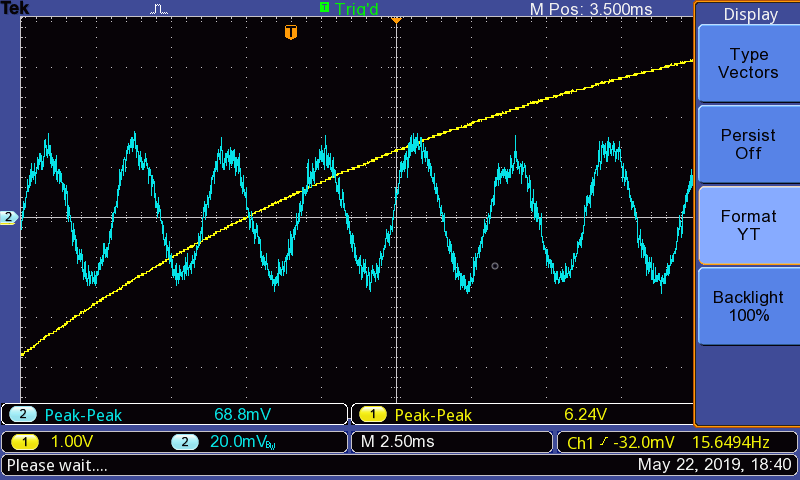
\includegraphics[scale=0.6]{Bilder/U_phi/oszi.png}
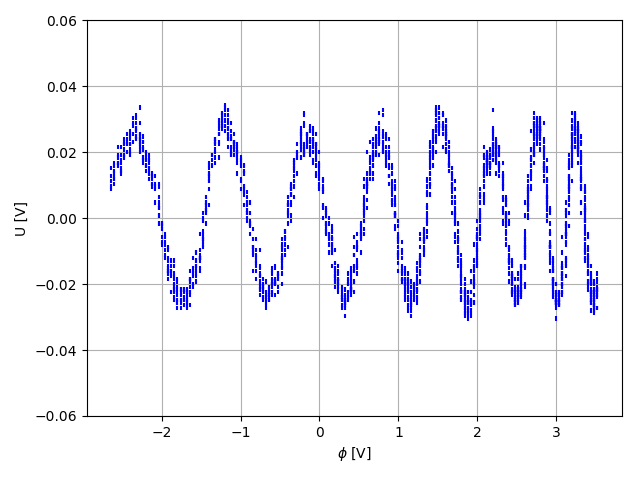
\includegraphics[scale=0.8]{Bilder/U_phi/data.png}
\caption{\textbf{top}: oscilloscope data recieved in the U-$\phi$ mode. The voltage is displayed in channel 2 and $\phi$ in channel 1. \textbf{bottom}: U-$\phi$ characteristic of the SQUID.}
\label{fig:U-phi_data}
\end{figure}

\subsection{Results}

\begin{figure}
\centering
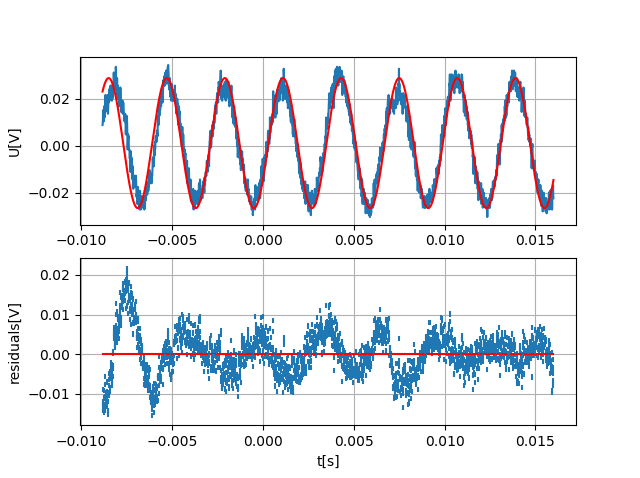
\includegraphics[scale=0.8]{Bilder/U_phi/fit.png}
\caption{sinus fit against the raw oscilloscope data.}
\label{fig:U-phi_fit}
\end{figure}

The U-$\si{\phi}$-characteristic is measured to determine the flux quantum. Theoretically this can be done by extracting the oscillation period from the characteristic, because each minimum should correspond to one flux quantum. However we have no way to calibrate the x-axis to the actual flux. So instead of analyzing the period we analyze the voltage difference between the minima and maxima.\\
This is done by fitting a function of the form
\begin{equation}
f(x) = a \cdot sin(b*x-c) + d
\label{eq:fit}
\end{equation}
against the raw oscilloscope data, as seen in figure \ref{fig:U-phi_fit}. The resulting fit values are listed in table \ref{tab:U-phi_fit}. There is a systematic oscillation visible in the residuals, which also results in an inaccurate frequency of the sinus fit, which is described by the parameter b. The method used for the fit requires starting parameters for a,b,c and d and the result is sensitive towards them. These parameters where chosen so that the error of a, which denotes the amplitude, is as small as possible. This results in an oscillation amplitude of:
\begin{equation}
a = \SI{0.0256\pm0.0006}{V}
\end{equation}
The error comes directly from the fit. However the sensitivity of the fit might introduce an additional error that was not analyzed.\\
The voltage displayed by the oscilloscope is amplified by a factor 10000. This means the real modulation amplitude is $2a/10000$:
\begin{equation}
\Delta V = \SI{5.12\pm 0.12}{\mu V}
\end{equation}
With this the SQUID-parameter $b_L$ can be determined:
\begin{equation}
b_L = \left(\dfrac{I_C R_n}{\Delta V}\right) -1 = 7.93\pm 0.22
\end{equation}
Finally the flux quantum can be extracted from $b_L$:
\begin{equation}
\phi_0 = 2 I_C \dfrac{L}{b_L} = \SI{2.10(6)e-15}{Wb}
\end{equation}
The inductance of the SQUID is approximated by $L = \SI{300}{pH}$.
The errors are derived from the errors of $I_C$, $R_n$ and $\Delta V$ by Gaussian error propagation.\\
The literature value of the flux quantum is $\Phi _0 = \SI{2.07e-15}{Wb}$. The measured value is comparable to this within its error range. However the inaccurate fit might introduce an additional systematic error in the result, which would further reduce the accuracy of the result to a point where its only comparable by coincidence.


\begin{table}
\center
\begin{tabular}{|c|c|c|c|c|}
\hline 
a & b & c & d & $\chi^2/dof$ \\ 
\hline 
$0.0256\pm0.0006$ & $196\pm 54$ & $0.6\pm0.4$ & $0.0011\pm0.0006$  & 1.75 \\ 
\hline 
\end{tabular}
\caption{Results of the sinus-fit from equation \ref{eq:fit}}
\label{tab:U-phi_fit}
\end{table}

\section{Qualitative Experiments}
As a final step a set of qualitative experiments was carried out to determine if objects in the vicinity of the SQUID can influence it. For this multiple objects of different materials were moved back and fourth close to the dewar and the U-I- and U-$\phi$-characteristics were observed on the oscilloscope for a reaction. The materials used are iron, nickel, copper, aluminum and plastic (carbon).\\
\\
This is first done with the magnetic shielding still in place. None of the materials induced a visible change in the characteristics, which means the magnetic shielding was efficient enough to nullify possible changes in the surrounding field. Turning the dewar also only increased the noise. This is however most likely related to the movement and not to changes in the magnetic field.\\
\\
The same experiment is then repeated without the magnetic shielding. For copper, aluminum and carbon there was still no change visible in the characteristics. However for iron a small phase change could be observed in the U-$\phi$-characteristic, as seen in figure \ref{fig:qual}. This indicates a change of the magnetic field measured by the SQUID. For nickel there was an even bigger phase shift of multiple oscillation periods.\\
The reactions to iron and nickel are not surprising, because both metals exhibit ferromagnetic properties and therefore influence the magnetic field directly. The other materials are not ferromagnetic and do not effect the magnetic field in a meaningful manner.\\
Turning the dewar or the SQUID inside also shows an effect, because the magnetic field from outside sources that penetrates the SQUID can change depending on its direction.

\begin{figure}
\centering
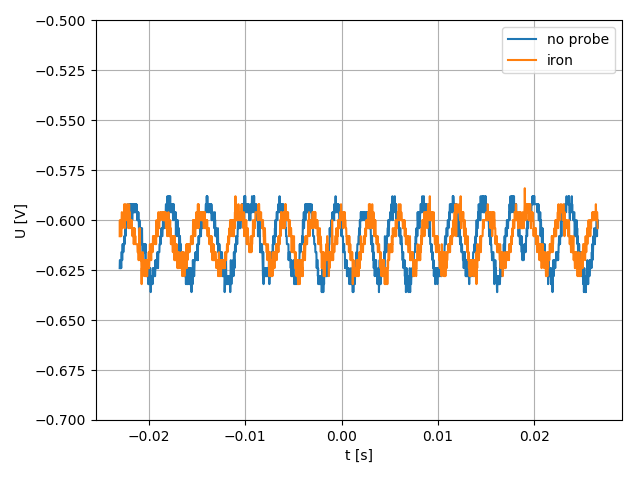
\includegraphics[scale=0.5]{Bilder/eisen.png}
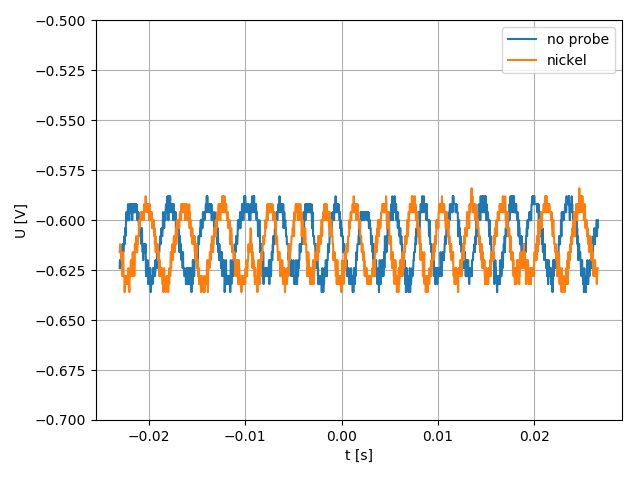
\includegraphics[scale=0.5]{Bilder/nickel.png}
\caption{U-$\phi$-characteristic observed when holding iron (left) and nickel (right) near the dewar. A phase change can be observed for both materials indicating a measured change in the magnetic field.}
\label{fig:qual}
\end{figure}
\section{Conclusion}
The measured temperature dependence of the SQUID resistance yielded the expected drop at the critical temperature, which could be determined with an accuracy of less than \SI{1}{K}. \\
The measurement of the U-I characteristic led to the expected behaviour with a plateau around zero and linear regimes before and after the plateau. With that it was possible to determine the values for the critical current, the resistance in the normal conductive regime and the characteristic voltage with an error of less than 1\%.\\
\\
The U-$\phi$-characteristic showed the expected voltage oscillation when changing the applied flux. The flux quantum has been determined by analyzing the amplitude of the oszillations and has a value of $\phi_0 =  \SI{2.10(6)e-15}{Wb}$ which matches the literature value within its error.\\
\\
Qualitative experiments also confirm, that the magnetic shielding is effective. Without the shielding both nickel and iron probes can influence the SQUID because of their ferromagnetic behavior. Non ferromagnetic probes have no effect on the SQUID.











\end{document}